\chapter{Boules, Intérieur, Adherence}

\justify

\setlength{\parindent}{0pt}
\renewcommand{\labelitemi}{\textbullet} % Utiliser des points noirs (•)

% ==================================================================================================================================
% Introduction

Maintenant que nous savons "mesurer" des "longueurs" et déterminer à quels points deux éléments d'un espace sont 
"proches", nous pouvons introduire de nouveaux object à la base de tous les raisonnements que nous auront par la suite. 

\vspace{0.3cm}

Ici, sauf mention contraire, nous nous plaçons dans un $\R$-espace vectoriel $E$. 
Pour toute partie $A$ de $E$, nous noterons son complémentaire dans $E$, $\overline{A}$, 
son adhérence $adh(A)$ et son intérieur $int(A)$. 

% ==================================================================================================================================
% Boules

\section{Boules}

Introduisons maintenant le concept de boule. 

\begin{definition}[Boule ouverte, fermée]
    Soit $a \in E, r \geqslant 0$ on appelle {boule ouverte} l'ensemble 
        \[ B(a,r) = \{ x \in E \; | \; \| x - a\| <  r\} \] 
    De même on définit la boule fermé comme l'ensemble :
    \[ \overline{B}(a,r) = \{ x \in E \; | \; \| x - a\| \leqslant r\} \] 
    On dit alors que $B(a,r)$ est la boule ouverte de rayon $r$ centrée en $a$ et 
    $\overline{B}(a,r)$ est la boule fermée de rayon $r$ centrée en $a$. 
\end{definition}

\begin{example}
    Pour tout $a \in \R$ on a :
        \[B(a,r) = \{ x \in E \; | \; \| x - a\| <  r\} = ]a - r ; a + r [ \]
        \[\overline{B}(a,r) = \{ x \in E \; | \; \| x - a\| \leqslant  r\} = [a - r ; a + r ] \]
\end{example}

\newpage 

\begin{remark}
    En fonction de la norme (ou de la distance) choisie, une même boule peut avoir plusieurs formes. 

    \begin{center}
        \begin{tikzpicture}[scale=1.1]
            % Norme 2 (cercle)
            \begin{scope}[xshift=-3cm]
                \draw[->] (-1.5,0) -- (1.5,0) node[anchor=north west] {$x_1$};
                \draw[->] (0,-1.5) -- (0,1.5) node[anchor=south east] {$x_2$};
                \fill[pattern=north east lines, pattern color=gray!50] (0,0) circle (1);
                \draw[thick,black] (0,0) circle (1);
                \node at (0,-1.8) {Norme $\|.\|_2$};
            \end{scope}
        
            % Norme 1 (losange)
            \begin{scope}[xshift=0cm]
                \draw[->] (-1.5,0) -- (1.5,0) node[anchor=north west] {$x_1$};
                \draw[->] (0,-1.5) -- (0,1.5) node[anchor=south east] {$x_2$};
                \fill[pattern=horizontal lines, pattern color=gray!50] (0,1) -- (1,0) -- (0,-1) -- (-1,0) -- cycle;
                \draw[thick,black] (0,1) -- (1,0) -- (0,-1) -- (-1,0) -- cycle;
                \node at (0,-1.8) {Norme $\|.\|_1$};
            \end{scope}
        
            % Norme infinie (carré)
            \begin{scope}[xshift=3cm]
                \draw[->] (-1.5,0) -- (1.5,0) node[anchor=north west] {$x_1$};
                \draw[->] (0,-1.5) -- (0,1.5) node[anchor=south east] {$x_2$};
                \fill[pattern=vertical lines, pattern color=gray!50] (-1,-1) rectangle (1,1);
                \draw[thick,black] (-1,-1) rectangle (1,1);
                \node at (0,-1.8) {Norme $\|.\|_\infty$};
            \end{scope}
        \end{tikzpicture}    
    \end{center}
\end{remark}

% ==================================================================================================================================
% Intérieur Adhérence

\section{Intérieur et Adhérence}

\begin{definition}[Intérieur]
    Soit $A \subset E$, soit $a \in E$, on dit que $a$ est intérieur à $A$ ssi 
        \[ \boxed { \exists \varepsilon > 0, \quad B(a,\varepsilon) \subset A } \] 
    Autrement dit, $a$ est intérieur à $A$ ssi on peut construire une boule autour de $a$ qui 
    soit entièrement contenue dans $A$. 

    On dit alors que $A$ est voisinnage de $a$. L'ensemble des points intérieurs d'une partie est appelé 
    l'intérieur de cette partie. On le note $int(.)$. 
\end{definition}

\begin{definition}[Adhérence]
    Soit $A \subset E$, soit $a \in E$, on dit que $a$ est adhérent à $A$ ssi 
        \[ \boxed { \forall \varepsilon > 0, \quad B(a,\varepsilon) \cap A \not = \emptyset } \] 
    Autrement dit, $a$ est adhérent à $A$ ssi pour toute boule autour de $a$, cette boule est intersectée avec $A$
    (i.e on ne peut pas construire de boule autour de $a$ qui ne "déborde" pas sur $A$).

    On dit alors que $a$ est dans l'adhérence de $A$. L'adhérence d'une partie est l'ensemble de ses points adhérents. 
    On le note $adh(.)$.
\end{definition}

\begin{remark}[Illustration]
    Soit $A \subseteq E$ et $x,y \in E$ tels que $x$ soit intérieur à $A$ et $y$ soit adhérent à $A$. 
    On pourrait représenter cela par le dessin ci-dessous :

    \begin{center}
        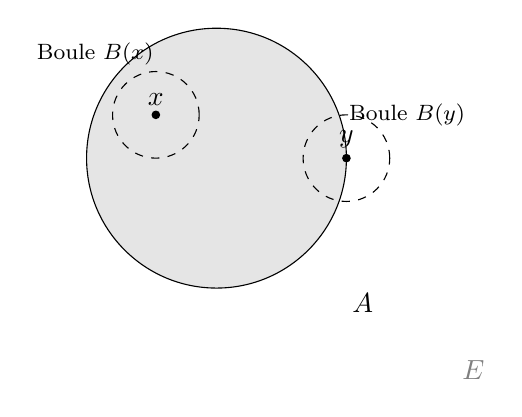
\begin{tikzpicture}[scale=1.1]
            % Partie A
            \draw[fill=gray!20,draw=black] (0,0) circle (1.5) node[below right=1.6cm, black] {$A$};
        
            % Point intérieur à A
            \fill[black] (-0.7,0.5) circle (0.05) node[above] {$x$};
            \draw[black, dashed] (-0.7,0.5) circle (0.5);
            \node[black] at (-1.4,1.2) {\footnotesize Boule ${B}(x)$};
        
            % Point adhérent à A mais pas intérieur
            \fill[black] (1.5,0) circle (0.05) node[above] {$y$};
            \draw[black, dashed] (1.5,0) circle (0.5);
            \node[black] at (2.2,0.5) {\footnotesize Boule ${B}(y)$};
        
            % Indication du fond (l'ensemble $E$)
            \node[below right=3cm, gray] at (0,0.5) {$E$};
        
            % Légendes
            % \draw[fill=blue!20, draw=blue, opacity=0.3] (-2.8,-2) rectangle (-1.8,-1.5);
            % \node[anchor=west] at (-1.7,-1.75) {\footnotesize Partie $A$};
            % \fill[red] (-2.8,-2.5) circle (0.1);
            % \node[anchor=west] at (-1.7,-2.5) {\footnotesize Intérieur ($x$)};
            % \fill[green] (-2.8,-3) circle (0.1);
            % \node[anchor=west] at (-1.7,-3) {\footnotesize Adhérent ($y$)};
        \end{tikzpicture}
    \end{center}

    L'intérieur d'une partie peut se voir comme l'ensemble des points "profonds" de cette partie. 
    Au contraire l'adhérence peut se voir comme tous les points qui sont dedans et "très proches". 
\end{remark}

\begin{definition}[Frontière]
    Soit $A \subseteq E$, on définit la frontière comme l'ensemble :
        \[ \partial A = adh(A) / int(A) \] 
\end{definition}

\begin{example}
    Soit $A$ le disque ouvert de rayon 1 dans $\R^2$. Déterminons son intérieur, son adhérence et sa frontière. 
        \[ A := \{ (x,y) \in \R^2 \; | \; x^2 + y^2 < 1 \} \] 
    On a : 
    \begin{itemize}
        \item $adh(A) = \{ (x,y) \in \R^2 \; | \; x^2 + y^2 \leqslant 1 \} $
        \item $int(A) = \{ (x,y) \in \R^2 \; | \; x^2 + y^2 \leqslant 1 \} = A $
        \item $\partial A = \{ (x,y) \in \R^2 \; | \; x^2 + y^2 = 1 \} $
    \end{itemize}
\end{example}


\subsection{Propriétés}

\begin{proposition}
    L'intérieur d'une boule ouverte est la boule fermée correspondante. 
\end{proposition}

\begin{prop}[Inclusions et complémentaire]
    Soit $E$ un espace métrique et $A,B \subseteq E$. 
    \begin{itemize}
        \item Si $A \subset B$ on a alors :
            \[ int(A) \subset int(B) \quad adh(A) \subset adh(B) \] 
        \item $int(A) = \overline{(adh(\overline{A}))} $ et $ adh(A) = \overline{(int(\overline{A}))}$ 
        \item 
        \begin{itemize}
            \item $ int(A \cup B) \supset int(A) \cup int(B) $
            \item $ int(A \cap B) = int(A) \cap int(B) $
            \item $ adh(A \cup B) = adh(A) \cup adh(B) $
            \item $ adh(A \cap B) \subset adh(A) \cap adh(B) $
        \end{itemize}
    \end{itemize}
\end{prop}

\begin{proposition}[Adhérence et sup dans le cas réel]
    Soit $A \subset \R$, non vide et majorée alors, $\sup (A) \in adh(A)$. 
\end{proposition}





